\chapter{Multiple Input Single Output Line Of Sight Channel}

this system uses a multiple antennas at the \Tx to decrease the probability of error in the communication system, and that's a type of Spatial Diversity.

\section{\Rx antenna array}
in a MISO communication system, we send the message from a \Rx with one antenna and receive it with multiable antennas \Tx.

the structure (the way the antennas are arranged) called the antenna array.
by using the two built-in functions 'phased.ULA' and 'getElementPosition', we can make a liner antenna array and get the coordinates for each antenna.


\subsection{Scatteringchanmtx}
as we did in SISO and SIMO LOS, we will repeat it for each system because we need scattering channel matrix to calculate the BER.
the difference here is we will replace the single antenna we put as the \Tx with the antenna array we made in the previous step.
and the \Rx will be one antenna as it was in SISO.

\section{Bit Error Rate (BER)}
we will calculate it this time for the MISO system.

to monitor the relationship between Eb/No and BER in a MISO LOS channel so will use the 11 values of Eb/No and calculate the BER for each one using helpMIMOBER function.

\vfill
\begin{figure}
	\centering
	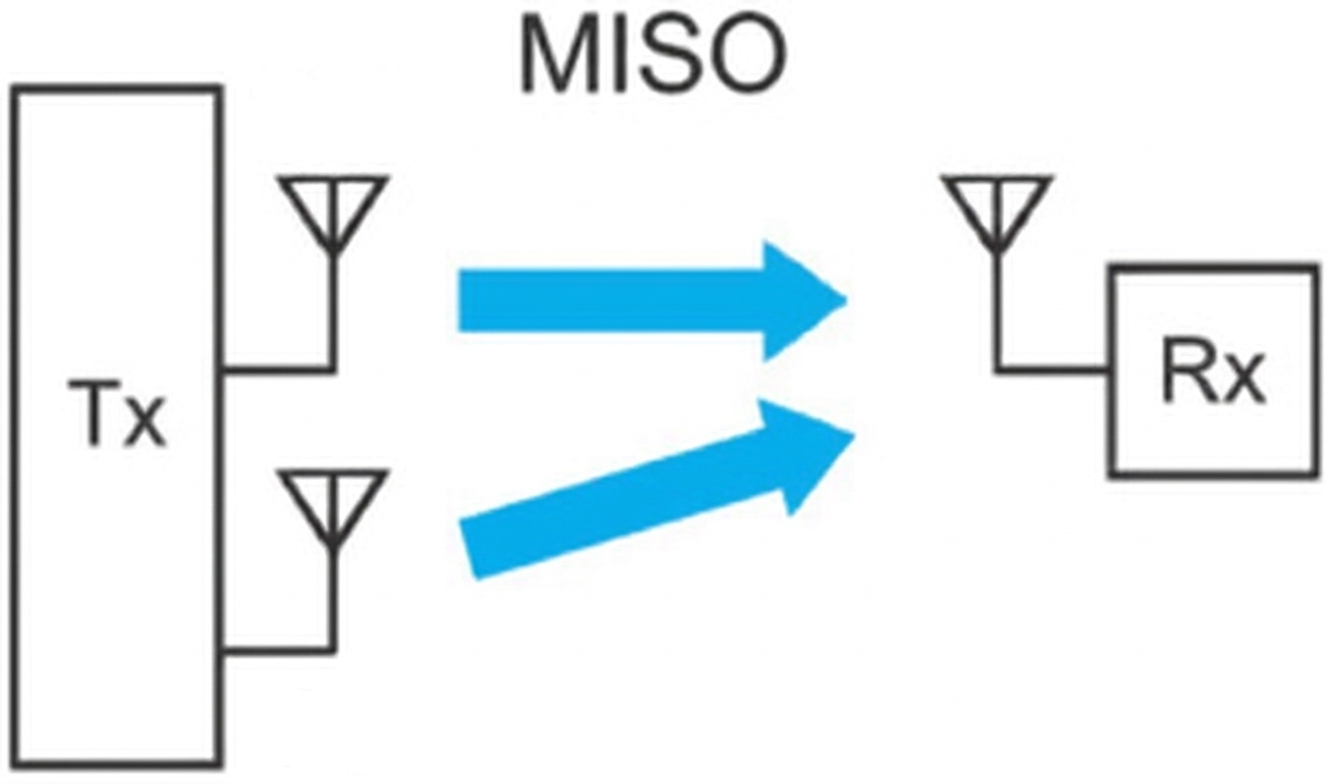
\includegraphics[width=0.4\linewidth]{figures/MISO-gem}
	\caption{MISO}
\end{figure}


\newpage
\section{Plotting}
to see the difference between SISO, SIMO and MISO we will plot all of them on the same graph.

as we can see in Figure[\ref{fig:sisosimomisober}], the BER decreases as we increase the Eb/No for each SISO, SIMO and MISO.

\section{Why do we see only two curves}
the graphs monitored on Figure[\ref{fig:sisosimomisober}] should have been three graph, because we are plotting 3 relations for three systems (SISO, SIMO and MISO).
but because the relation between Eb/No and BER for SIMO and MISO are identical, they overlap each other so we can only see SISO curve and the overlapping SIMO, MISO curev.


\begin{figure}[!h]
	\centering
	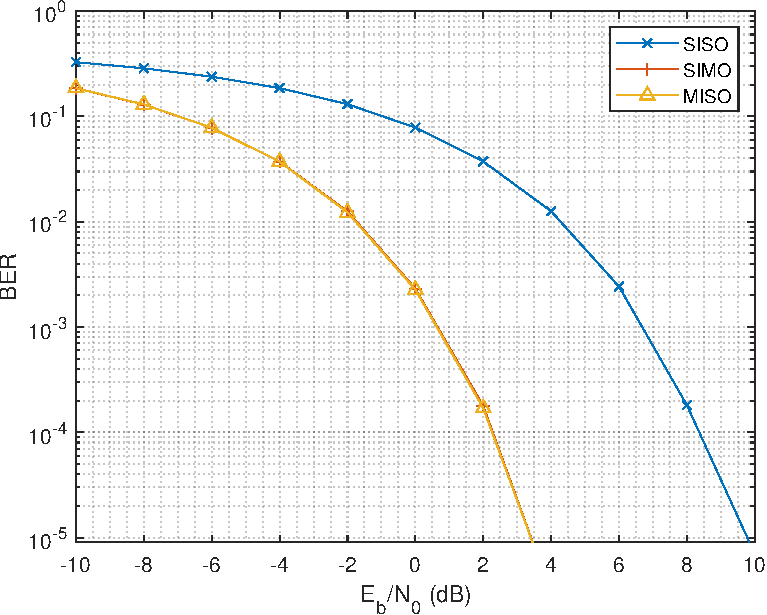
\includegraphics[width=1\linewidth]{figures/SISO_SIMO_MISO_BER}
	\caption{}
	\label{fig:sisosimomisober}
\end{figure}



\newgeometry{margin=0pt}
\newpage
\vfill
\begin{figure}
	\centering
	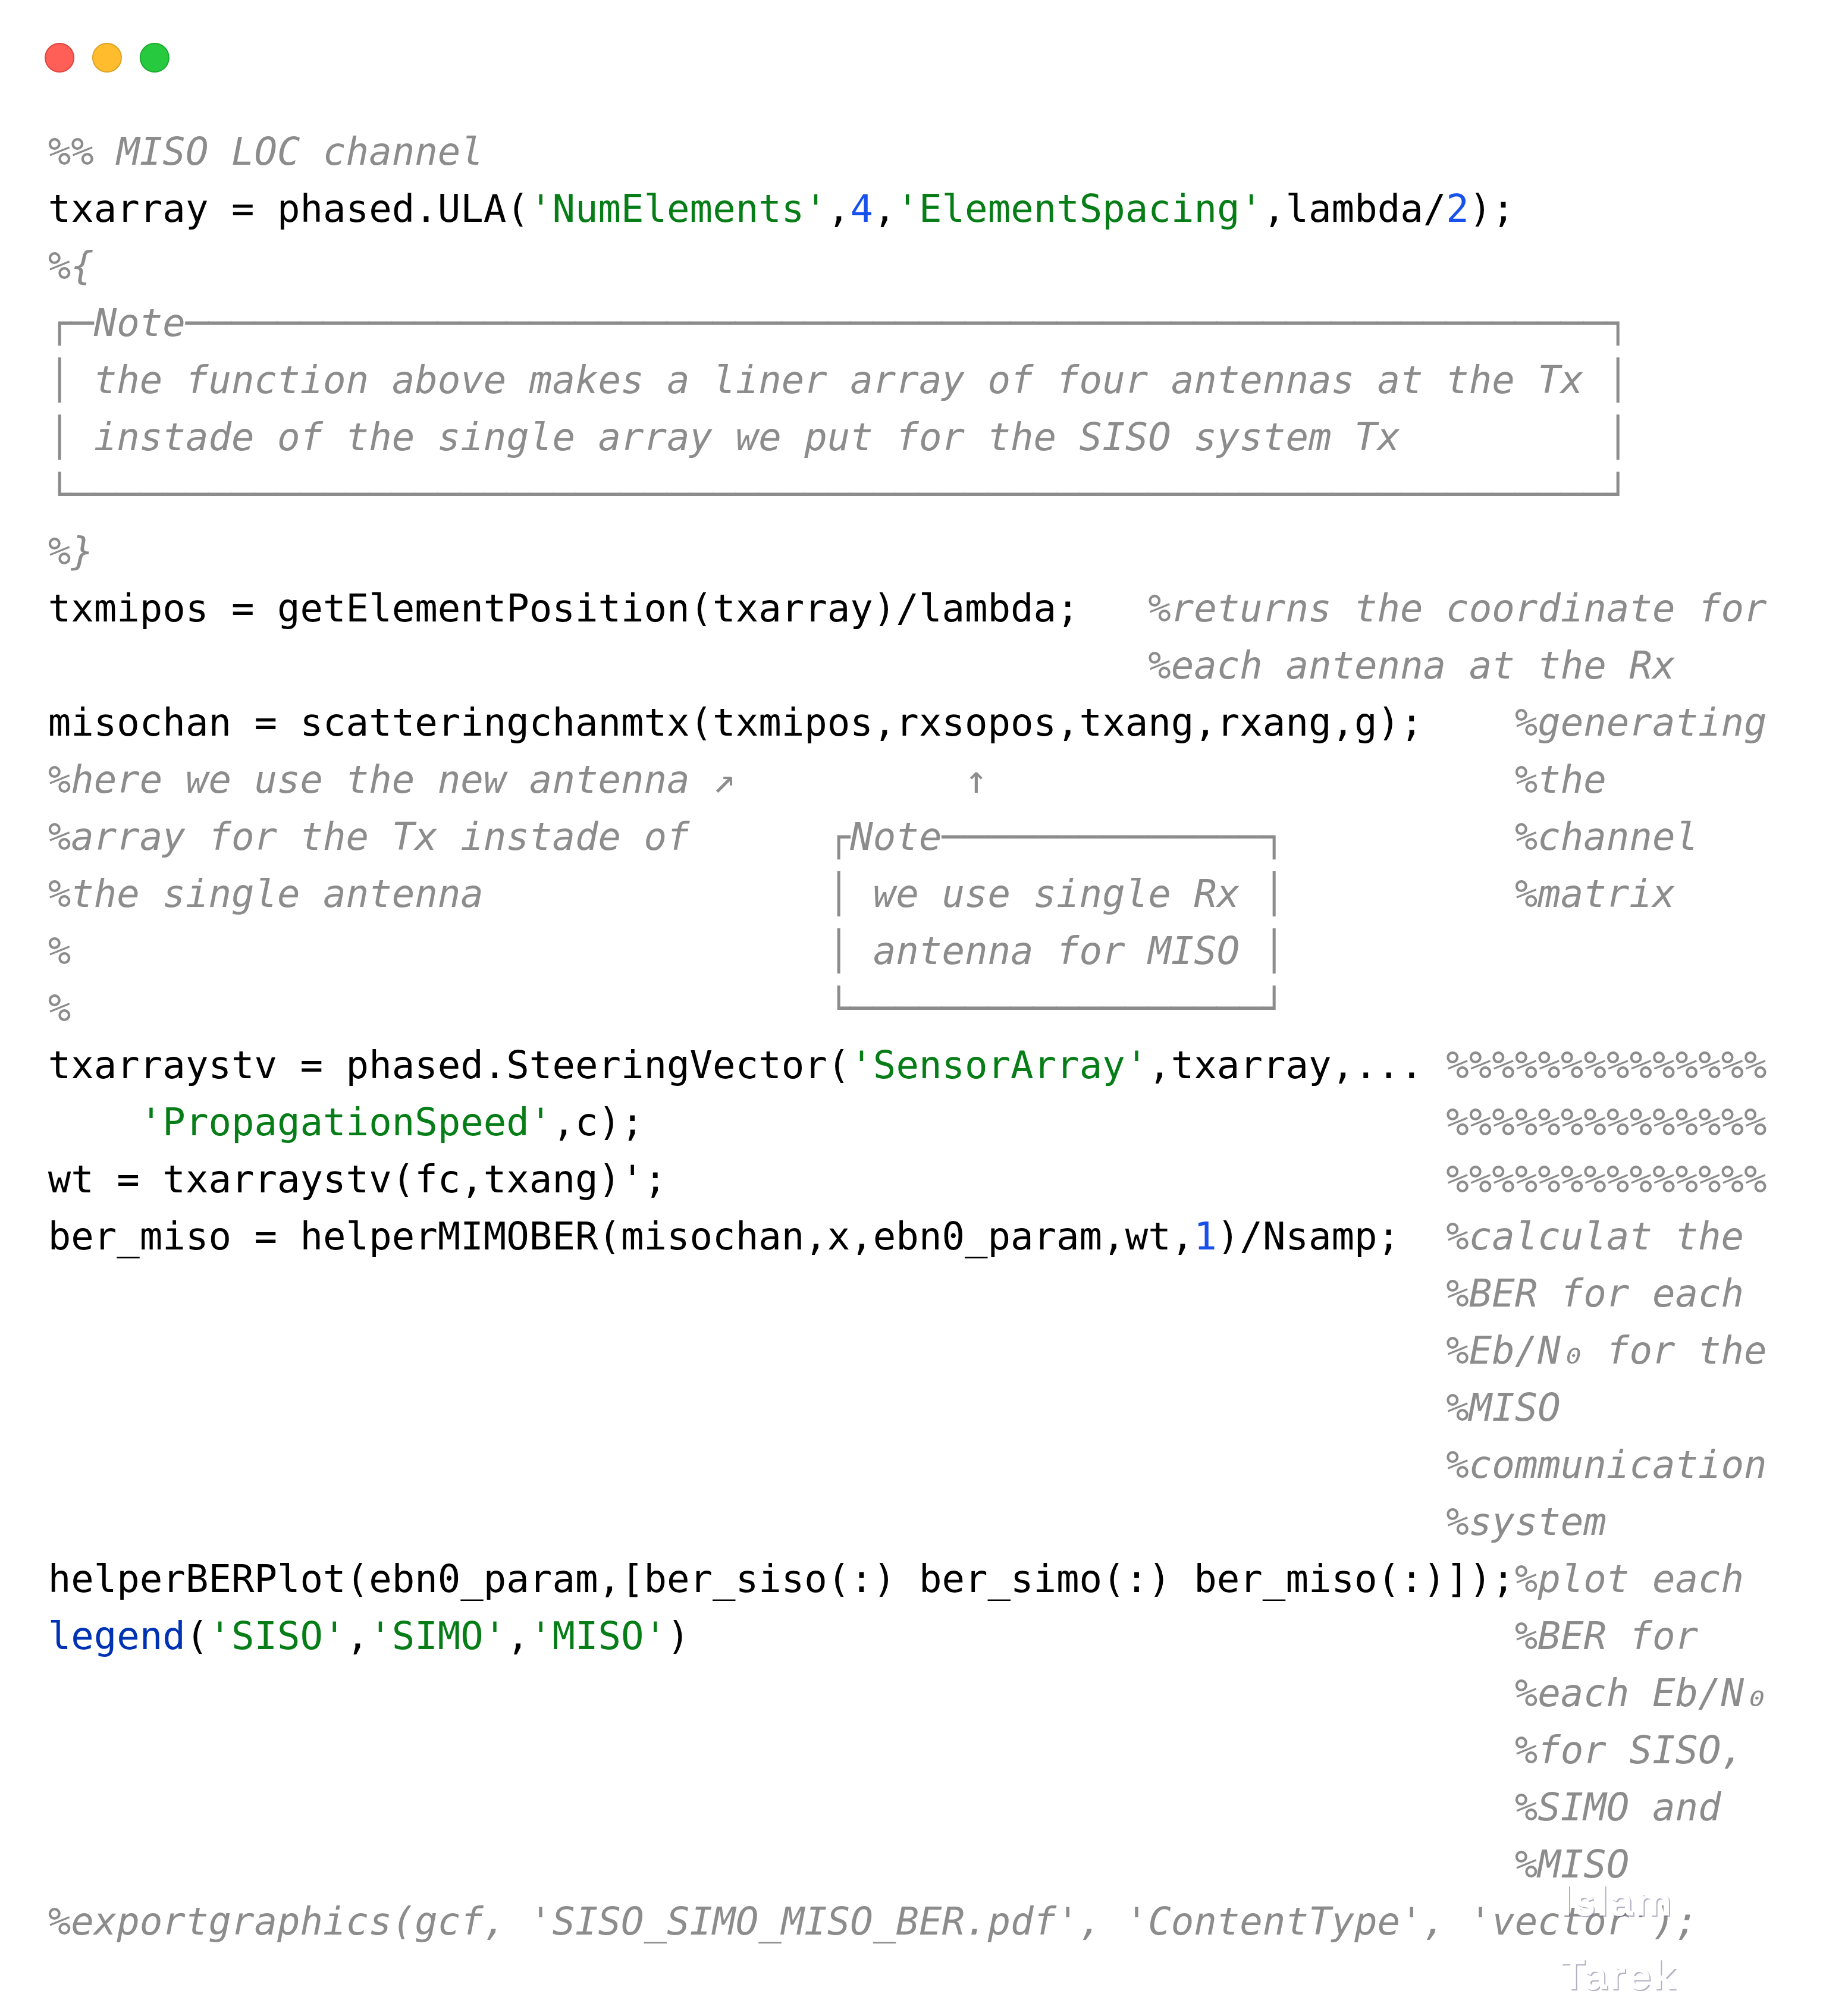
\includegraphics[width=0.7\linewidth]{figures/code4}
\end{figure}
\vfill
\restoregeometry